\documentclass{article}

\usepackage[italian]{babel}
\usepackage[utf8]{inputenc}
\usepackage[pdftex]{graphicx}
\graphicspath{{img/}}
\usepackage{epstopdf}
\usepackage{hyperref}  %% conviene compilare più volte con questo comando, per far funzionare tutto!

%\usepackage[scale=0.5]{geometry}
\usepackage{caption}
\usepackage{subfig}



\author{Nome dell'autore}
\title{\textbf{La gestione delle immagini}}
\date{\today}

\begin{document}

\maketitle
\tableofcontents
\listoffigures


\section{Da sole}
\begin{figure}[h]
	\centering
	
\includegraphics{AIM}
	\caption{La nostra prima immagine...}
	\label{img:logo}
\end{figure}

\section{Nel testo}
Proviamo ora a inserire una immagine qui 
\includegraphics{AIM}. Anche per le immagini è possibile creare dei riferimenti (ad esempio vedi \autoref{img:logo}).

\section{Con minipage}
\begin{minipage}[t]{.5\linewidth}
	\centering
	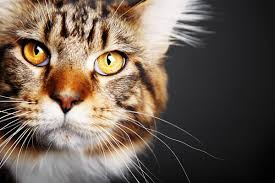
\includegraphics[width = .9\linewidth]{cat1}\label{img:cat1}
	\captionof{figure}{Ed ora, gatti...}
\end{minipage}
\hfill
\begin{minipage}[t]{.5\linewidth}
	\centering
	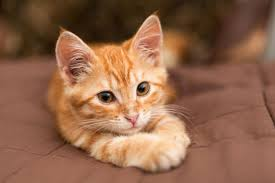
\includegraphics[width = .9\linewidth]{cat2}\label{img:cat2}
	\captionof{figure}{Ancora gatti...}
\end{minipage}

\vspace{.5cm}
\noindent
Alcuni consigli e accorgimenti per un corretto uso di minipage e immagini (ovvero, come non impazzire cercando di far produrre a LaTeX ciò che vogliamo):
\begin{itemize}
	\item l'uso dell'ambiente \verb|figure| all'interno di \verb|minipage| non è in generale consentito per ragioni tecniche (un \emph{floating-object} dentro un oggetto che \emph{floating} non è...); una possibile soluzione è
	\begin{enumerate}
		\item non usare del tutto \verb|figure|, e inserire il pacchetto \verb|caption| per avere le didascalie correlate alle immagini
		\item utilizzare \verb|minipage| all'interno di \verb|figure|;
		\item utilizzare \verb|subfloat|, che permette anche più flessibilità;
	\end{enumerate}
	\item disporre le immagini in maniera coerente con il contenuto circostante migliora la fruizione di un documento!
\end{itemize}

\section{Con subfloat}
\begin{figure}[h]
	\centering
	\subfloat[][posso anche aggiungere...]
	{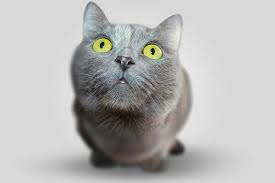
\includegraphics[width = .45\linewidth]{cat3}\label{img:cat3}}
%	\hspace{0.05\linewidth}
	\hfill
	\subfloat[][... didascalie parziali!]
	{
\includegraphics[width = .45\linewidth]{cat4}\label{img:cat4}}
	\caption{Sempre gatti...}
\end{figure}
\noindent
In questo caso abbiamo allineato la Figura \ref{img:cat3} con la Figura \ref{img:cat4} utilizzando il comando \verb|\subfloat|;\\ la spaziatura tra le immagini non c'è di default, va inserita ad hoc con i comandi \verb|\hspace{??cm/inch/pt/...}| o \verb|\hfill|

\end{document}
